% Created 2018-04-09 Mon 11:11
% Intended LaTeX compiler: pdflatex
\documentclass[10pt]{beamer}
\usepackage[utf8]{inputenc}
\usepackage[T1]{fontenc}
\usepackage{graphicx}
\usepackage{grffile}
\usepackage{longtable}
\usepackage{wrapfig}
\usepackage{rotating}
\usepackage[normalem]{ulem}
\usepackage{amsmath}
\usepackage{textcomp}
\usepackage{amssymb}
\usepackage{capt-of}
\usepackage{hyperref}
\usetheme{Boadilla}
\author{ECON 499: Growth and Development}
\date{Spring 2018}
\title{Physical Capital}
\usecolortheme{seagull}
\usefonttheme[onlylarge]{structurebold}
\usefonttheme[onlymath]{serif}
\setbeamerfont*{frametitle}{size=\normalsize,series=\bfseries}
\setbeamertemplate{navigation symbols}{}
\setbeamertemplate{itemize item}[triangle]
\setbeamertemplate{footline}{}
\setbeamertemplate{enumerate items}[default]
\hypersetup{
 pdfauthor={ECON 499: Growth and Development},
 pdftitle={Physical Capital},
 pdfkeywords={},
 pdfsubject={},
 pdfcreator={Emacs 25.2.2 (Org mode 9.1.6)}, 
 pdflang={English}}
\begin{document}

\maketitle

\begin{frame}[label={sec:org32451db}]{}
\begin{itemize}
\item Reading
\begin{itemize}
\item Textbook, chapter 3
\end{itemize}

\item Homework
\begin{itemize}
\item On Canvas
\end{itemize}

\item Next class
\begin{itemize}
\item Bexell 120 (we'll work on the homework)
\end{itemize}
\end{itemize}
\end{frame}

\begin{frame}[label={sec:org0948660}]{}
\alert{Physical capital}
\begin{itemize}
\item Capital is a collection of things that workers use to produce output
\item Workers can produce more with capital than without it
\item Countries with more capital can produce more, have higher income
\end{itemize}
\end{frame}

\begin{frame}[label={sec:org16b7b57}]{}
\begin{center}
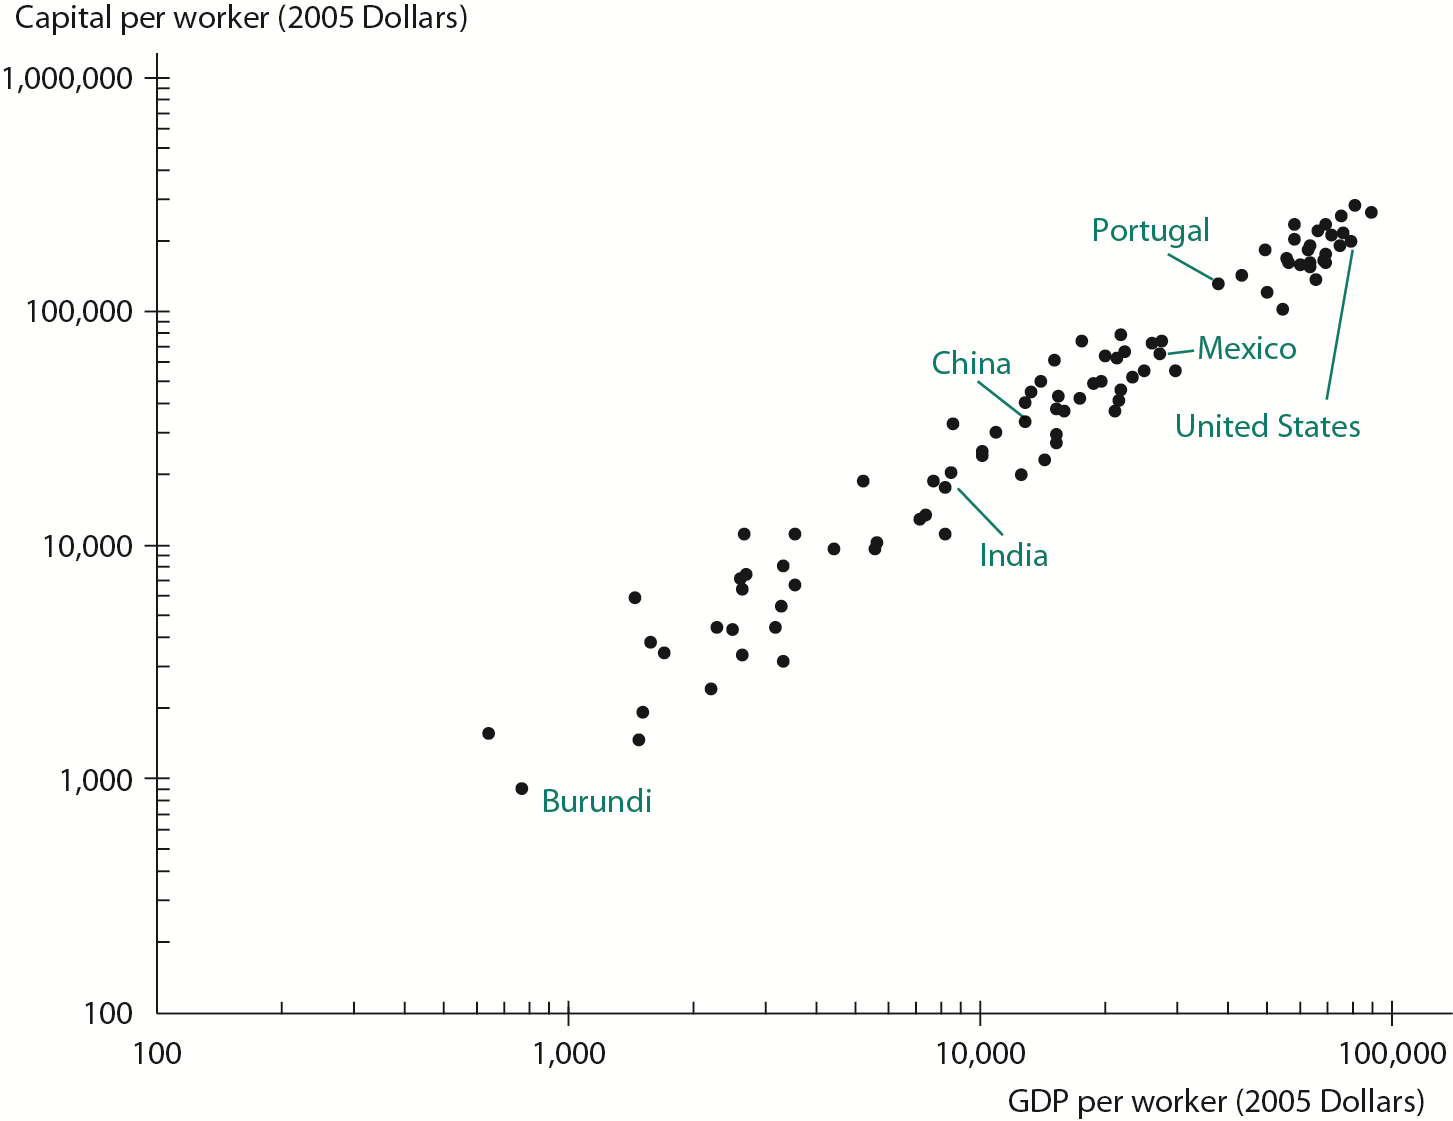
\includegraphics[width=.75\textwidth]{./img/3.1.png}
\end{center}
\end{frame}

\begin{frame}[label={sec:org0a5805b}]{}
\alert{Properties of capital}
\begin{itemize}
\item Capital is:
\begin{enumerate}
\item Productive
\item Produced
\item Rival
\item Depreciating
\end{enumerate}
\end{itemize}
\end{frame}

\begin{frame}[label={sec:org6a5e3b8}]{}
\alert{Productive capital}
\begin{itemize}
\item Workers use capital to produce goods and services (machines, tools, factories, etc)
\item More capital means workers are more productive
\item Increasing capital per worker \(\rightarrow\) increasing output per worker \(\rightarrow\) increasing income per worker
\end{itemize}
\end{frame}

\begin{frame}[label={sec:org78bb0ac}]{}
\alert{Investment}
\begin{itemize}
\item Capital is itself produced by a production process
\item Only things that are produced are capital (land is not capital)
\item Resources that are used to produce capital are called \emph{investments}
\item There is a tradeoff between producing consumption goods and capital
\item Consumers (and governments) either consume or save, therefore savings=investment (Keynesian IS curve)
\end{itemize}
\end{frame}

\begin{frame}[label={sec:orgd69e4a5}]{}
\alert{Rivalry}
\begin{itemize}
\item If a hammer is being used by one worker, it cannot be used by another worker
\item Capital has a finite capacity, not every worker can use the same capital equipment
\end{itemize}
\end{frame}

\begin{frame}[label={sec:org1d2561e}]{}
\alert{Depreciation}
\begin{itemize}
\item Capital wears out (depreciates) over time
\item Tools break, machines need maintenance, etc
\item Some continued investment is needed to maintain a level of capital
\end{itemize}
\end{frame}

\begin{frame}[label={sec:org720df37}]{}
\alert{The production function}
\begin{itemize}
\item Workers use capital to create consumption goods and services (and capital)
\item A production function describes the way in which labor and capital can be combined to create output goods
\item In mathematics, a \emph{function} transforms inputs (labor, capital) into output (GDP)
\end{itemize}

$$Y=F(K,L)$$
\end{frame}

\begin{frame}[label={sec:org57dbbaa}]{}
\alert{Assumptions}
\begin{itemize}
\item Constant returns to scale (CRS):
\end{itemize}
$$F(zK,zL) = zF(K,L)$$
\begin{itemize}
\item Diminishing marginal product: MPK and MPL diminish as additional units are added
\end{itemize}
\end{frame}
\end{document}